

\documentclass[runningheads]{llncs}

\usepackage{hyperref}
\usepackage{graphicx}
\usepackage{afterpage}
\usepackage{caption}

\title{Pristine Sentence Translation: A New Approach to a Timeless Problem}

\author{
	Meenu Ahluwalia, Brian Coari, and Ben Brock
}

\institute{$^1$Master of Science in Data Science \\ Southern Methodist University \\ Dallas, Texas USA \\
	\email{\{mahluwalia, bcoari, bbrock\}@smu.edu}}


\begin{document}
	
	\maketitle
	
	\begin{abstract}
		Translating text from one language to another is a continuous technological challenge. Although many technologies, such as Google Translate, have used machine learning and neural networks to close the translation gap, there are still many translation problems to be solved. Issues such as multiple word meanings, proper sentence structure, slang, colloquialisms, and determining the literal meaning of words vs contextual intent of those words are areas where we sometimes still see Google Translate struggle. In this paper we explore an original strategy that provides a solution to these translation issues, demonstrate a proof-of-concept of the solution, and examine the feasibility of a large-scale solution. For our translation solution we populated a database with translations of entire sentences from one language to another, instead of the words in a sentence. Since a sentence represents an entire thought instead of an assembly of words, the translation did not suffer from the issues that plague Google Translate. We also used Natural Language Processing (NLP) and predictive modeling in order to find sentences close to the sentence requested, which provides the user examples of common grammatically-correct sentences. With these approaches we were able to translate sentences that seemed impossible using traditional translation methods.
		
	\end{abstract}
	
	%\begin{keywords}
	%Data Science, Predictive Analytics, NLP, Translation, Goodle Cloud
	%\end{keywords}
	
	\section{Introduction}
	
	The ability to easily communicate with people in another language is one of the most powerful and satisfying experiences in life. Technology has come a long way from the discovery of the Rosetta Stone in 1799, which allowed us to translate Egyptian hieroglyphics to ancient Greek in a mere 23 years. In the modern day, tools such as Google translate can be used in real time to convert between languages and allow people to connect from different cultures~\cite{ref_url6}. The latest iterations of Google Translate even use machine learning and neural nets to parse more than just  single words, delivering a more satisfying user experience~\cite{ref_url7}.
	
	As far as we have come, however, the areas where we struggle are still painfully obvious. While Google Translate will usually allow you to find a bathroom and order off a menu, the intricacies and complexities of a normal, native conversation still can cause a non-fluent speaker issues. For example, if an American coworker mentions to a Brazilian coworker about their performance on a project with "You hit one out of the park.", the Brazilian coworker could translate the words, but without familiarity with the context of a baseball game, the Brazilian would be confused and would have to ask for clarification if it was possible. It would be even harder if the Brazilian was reading a book in English with a colloquialism, since there would be no human to ask for help.
	
	If you consider these kinds of issues from a high level they might seem unsolvable. How can you train a translation tool to look at the meaning behind sentences using on the words provided? We think we have a possible answer: an original concept we are calling Pristine Sentence Translations (PSTs). The concept of PST is that instead of translating words or phrases using neural nets and machine learning, we simply store an entire sentence in a database, and we have entire sentences in other languages that represent the meaning of that sentence. 
	
	For example, using the example above we would have an entry for the English sentence "You hit one out of the park", and we would have an entry for a Portuguese sentence mapped to that English sentence that says "Você foi ótima" which translates in English to the meaning behind the phrase: "You did great". For another example, in Portuguese there's a sentence "Eu adoro Cafuné" Google Translate does not have a translation for "Cafuné", because it's a complicated word which loosely means "the act of running fingers through hair" . Our program's goal is to return an English translation "I love the feeling of fingers running through my hair" when asked to translate "Eu adoro Cafuné" into English. Using this method there is no sentence or concept we will not be able to translate into another language given enough time and resources.
	
	One main issue with the approach outlined above is that if we do not have an exact match for the sentence, our method return nothing. so if we tried to translate "You really hit one out of the park" from English into Portuguese we would not get any results. We decided to address this concern using Natural Language Processing (NLP) to filter out the noise in a sentence, and then use Predictive Modeling in order to find the sentence "most like" the input sentence. Using this method, "You really hit one out of the park" would ideally map most closely to "You hit one out of the park", and return the same translation: "Você foi ótima". The front-end will indicate that the translation is not for the original input sentence, instead it will indicate that it is "Showing Results for: You hit one out of the park."
	
	Due to the strictly educational and academic nature of the project, we are not attempting to provide a full translation solution. We will limit our translations to English, Portuguese, and Hindi, and we will only provide translations for a few hundred phrases. This will be sufficient to demonstrate the appeal and power of this technique, and we will show how this solution could grow into a complete, living solution using crowdsourcing and time. 
	
	\section{State of Translations}
	Meenu or Brian - Meenu to pick either "State of Translations" or "A New Approach to Translations"
	
	\subsection{Existing Tools and Methods}
	
	\subsection{Outstanding Issues}
	
	\section{A New Approach to Translations}
	Meenu or Brian - Meenu to pick either "State of Translations" or "A New Approach to Translations"
	
	\subsection{Pristine Sentence Translations Theory}
	
	\subsection{Pristine Sentence Translations In Action}
	
	\subsection{Database Design}
	
	\section{Predictive Modeling}
	Meenu citing https://machinelearningmastery.com/develop-neural-machine-translation-system-keras/
	
	Automatic or machine translation is one of the most challenging AI tasks given the fluidity of human language. Classically, rule-based systems were used for this task, which were replaced in the 1990s with statistical methods. More recently, deep neural network models achieve state-of-the-art results in a field that is aptly named neural machine translation. 
	
	Sequence to Sequence (often abbreviated to seq2seq) models are a special class of Recurrent Neural Network architectures typically used (but not restricted) to solve complex Language related problems like Machine Translation, Question Answering, creating Chat-bots, Text Summarization, etc. Our aim is to translate given sentence from one language to another. We will target sentence translations to and from English, Portuguese and  Hindi languages only. Use of seq2seq (or Encoder-Decoder) architecture is appropriate in this case as the length of the input sequence  does not has the same length as the output data
	
	To summarize our model, the Encoder simply takes the input data, and train on it then it passes the last state of its recurrent layer as an initial state to the first recurrent layer of the decoder part. The Decoder takes the last state of encoder’s last recurrent layer and uses it as an initial state to its first recurrent layer , the input of the decoder is the sequences that we want to get. We will use Keras API with Tensorflow backend to build our model.


	\subsection{Data Preparation}
	Before we start building the model, we need to clean up the text data (i.e. the sentences). We will remove all punctuation characters, normalize the case to lowercase, normalize all Unicode characters to ASCII and remove any tokens that are not alphabetic. To build the model, we need to map words to Integers. We will use Keras Tokenize class for this. The Tokenizer must be constructed and then fit on either raw text documents or integer encoded text documents. Once fit, the Tokenizer provides four attributes that you can use to understand about your text., viz.,
					\begin{enumerate}
						 \item word-counts: A dictionary of words and their counts
						 \item word-docs: A dictionary of words and how many documents each appeared in.
						\item word-index: A dictionary of words and their uniquely assigned integers.
						\item document-count:An integer count of the total number of documents that were used to fit the Tokenizer.
					\end{enumerate}
	
	We will also compute the vocabulary sizes and the length of maximum sequence for both the languages. We need to encode each input and output sentences to integers and  pad them to the maximum phrase length to make all sentences of the same length. This is because we will use word embedding for the input sentence and one hot encoding for the output. In one hot encoding, a document is represented as a sequence of integer values, where each word in the document is represented as a unique integer. One hot encoding is needed because the model will predict the probability of each word in the vocabulary as output.
	

	
	\subsection{Encoder-Decoder Long Short-Term Memory (LSTM) Networks}	
	A typical seq2seq model consists of 2 major components
	\begin{enumerate}
		\item Encoder
		\item Decoder
	\end{enumerate}
	
	Both these components are essentailly two different Recurrent Neural Network models combined into one giant network.
	
	\begin{minipage}{\linewidth}
		\begin{center}
			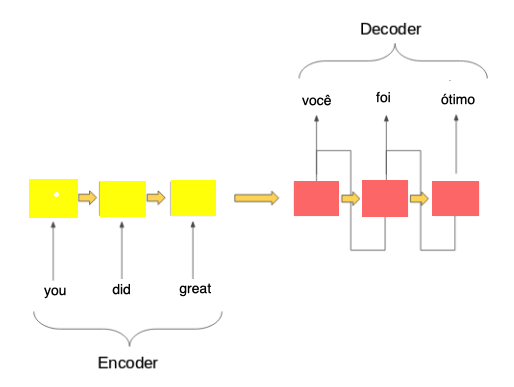
\includegraphics[width=\linewidth]{enc_dec_2.png}
			\captionof{figure}{Sequence to Sequence Modell}
			\label{fig:Sequence to Sequence Model}~\cite{ref_url4}
		\end{center}
	\end{minipage}
	\afterpage{\clearpage}
	
	We will explain the  Encoder and Decoder model in more detail.  
	
	Let's say we are trying to convert the following sentence from English to Portuguese.

	Input sentence (English) - i have lost my passport
	
	Output sentence (Portuguese) - eu perdi meu passaporte
	
	A sentence can be seen as a sequence of words or characters. We will split the sentence by words. So, for the above example in English, there are 5 words which are fed to the encoder as shown in the figure below. The input is referred to as X and X{i} is the input sequence at time step i. So we have the following input.
	X{1} = i, X{2} = have, X{3} = lost,  X{4}=my, X{5} = passport.
	Each X{i} is mapped to a fixed-length vector using the built-in embedding layer of Keras API.
	
	The LSTM will read this sentence word by word in 5 time steps as shown in the figure.
	
	\begin{minipage}{\linewidth}
		\begin{center}
			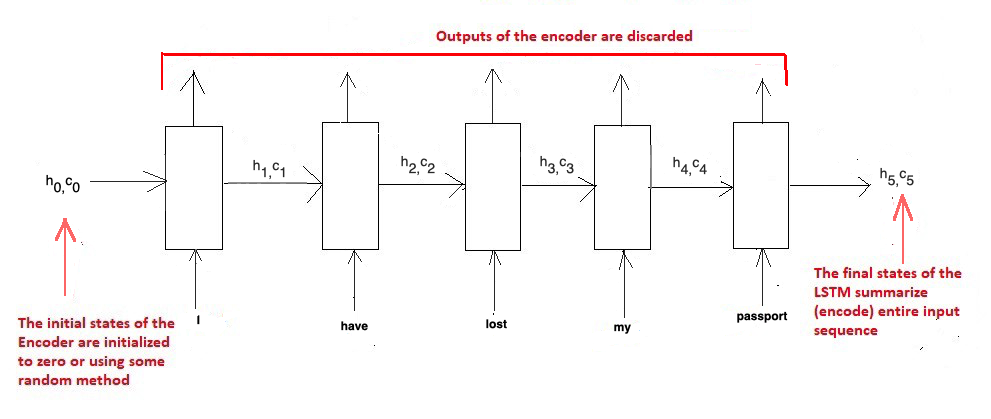
\includegraphics[width=\linewidth]{EncoderLSTM.jpeg}
			\captionof{figure}{Encoder LSTM}
			\label{fig:Encoder LSTM}~\cite{ref_url5}
		\end{center}
	\end{minipage}
	\afterpage{\clearpage}
	
 	h{i} and c{i} in the figure above represent the internal state, viz., the hidden state and the cell state of the Encoder. In simple terms, they remember what LSTM has read till now. 
 	For example, 
 	h{3}, c{3} vectors will remember that the network has read “I have lost” till now. Basically its the summary of information till time step 3 which is stored in the vectors h3 and c3 (thus called the states at time step 3). So, h{5},c{5} will contain the summary of the entire sentence. These states coming out of the last time step are also called as the “Thought vectors” as they summarize the entire sequence in a vector form. We initialize h{0},c{0} to zero as the model has not started to read the input.
 	
 	Y{i} is the output of the LSTM at each step. We discard the outputs of the encoder and only preserve the internal states as the model has nothing to output unless it has read the entire English sentence.
	
	Next, we define the Decoder. Unlike the Encoder LSTM which has the same role to play in both the training phase as well as in the inference phase, the Decoder LSTM has a slightly different role to play in both of these phases. Recall that given the input sentence "i have lost my passport", the goal of the decoder is to output "eu perdi meu passaporte". 

	The intial states (h{0},c{0}) of the Decoder are set to the final states of the Encoder. This intuitively means that the decoder is trained to start generating the output sequence depending on the information encoded by the encoder.
	
	\begin{minipage}{\linewidth}
	 	\begin{center}
	 		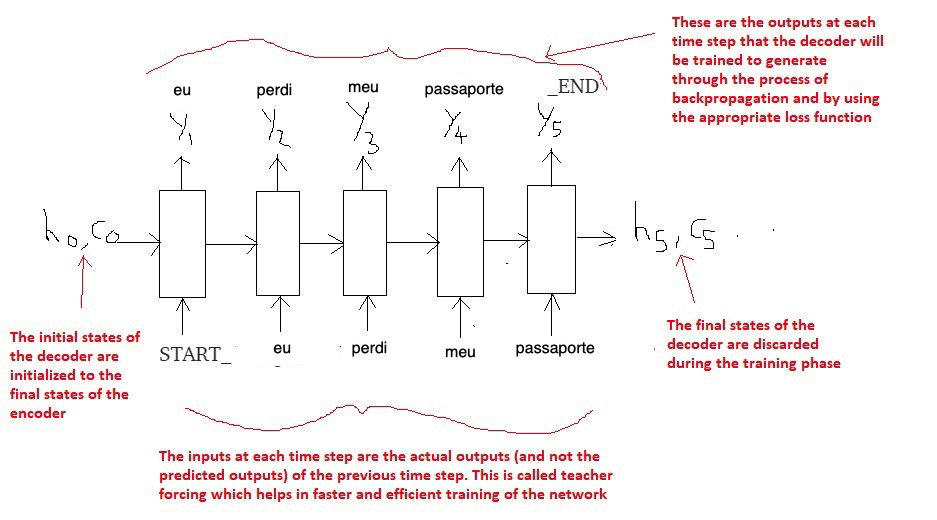
\includegraphics[width=\linewidth]{decoder.jpeg}
	 		\captionof{figure}{Decoder LSTM}
	 		\label{fig:Decoder LSTM}~\cite{ref_url6}
	 	\end{center}
	 \end{minipage}
	 \afterpage{\clearpage}
	 
	\subsection{Building the Neural Translation Model}
	We will split our dataset into train and test set for model training and evaluation, respectively.
	Our seq2seq model is defined as the following

	\begin{enumerate}
		\item For the encoder, we will use an embedding layer and an LSTM layer
		\item For the decoder, we will use another LSTM layer followed by a dense layer
	\end{enumerate}

	\begin{minipage}{\linewidth}
		\begin{center}
			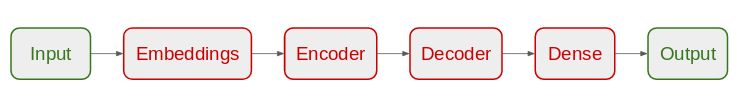
\includegraphics[width=\linewidth]{architecture.png}
			\captionof{figure}{Model Architechture}
			\label{fig:Model Architectture}~\cite{ref_url7}
		\end{center}
	\end{minipage}
	\afterpage{\clearpage}


	To be continued....
	
	
	\subsection{Evaluating the Neural Translation Model}
	
	\section{Full Demo}
	The front end for the Pristine Language Translation (PST) site is a simple proof-of-concept page with three boxes for input: The language and the text the user is translating from, and the language code the user is translating to. The user must fill in all three boxes with valid input before hitting the "Translate" button:

	\begin{minipage}{\linewidth}
		\begin{center}
			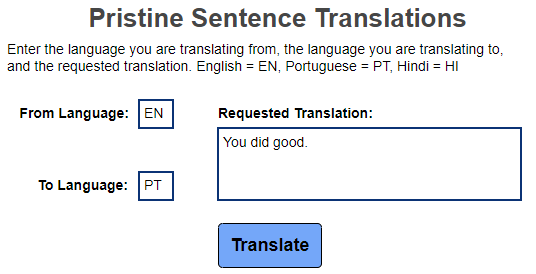
\includegraphics[width=\linewidth]{Screen_top.png}
			\captionof{figure}{Language Input}
			\label{fig:Language Input}
			\vspace*{1cm}
		\end{center}
	\end{minipage}
	\afterpage{\clearpage}
After the user has entered the data and hit the "Translate" button the information is passed to our pyton NLP processing. First our model finds the closest linguistic match to the sentence entered to a sentence for which the translation is known. Then we have a separate pos-processing step to calculate how close of a match the input sentence is to the matched sentence, and we retrieve that translations of that sentence for the requested language:

	\begin{minipage}{\linewidth}
		\begin{center}
			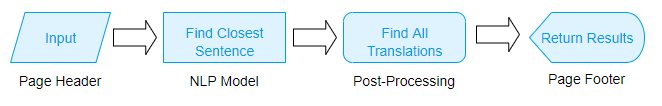
\includegraphics[width=\linewidth]{Process_Map.png}
			\captionof{figure}{Process Map}
			\label{fig:Process Map}
			\vspace*{1cm}
		\end{center}
	\end{minipage}
	\afterpage{\clearpage}
The results are then reurned to the screen for display. Note that there can be more than one valid translation for an input sentence, provided our database has the mappings:

	\begin{minipage}{\linewidth}
		\begin{center}
			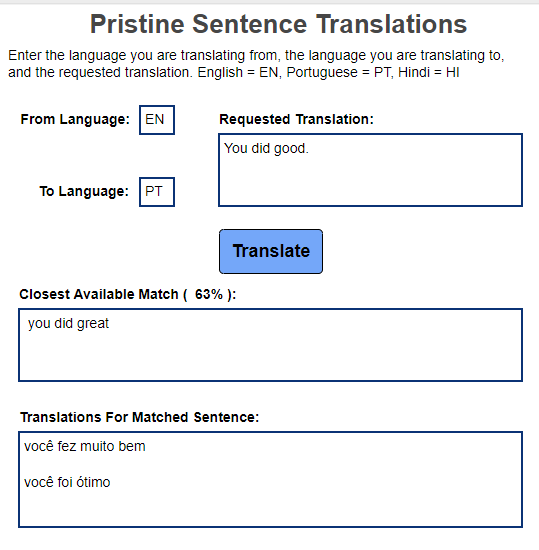
\includegraphics[width=\linewidth]{Screen.png}
			\captionof{figure}{Display Translations}
			\label{fig:Display Translations}
			\vspace*{1cm}
		\end{center}
	\end{minipage}
	\afterpage{\clearpage}
If the user wants to try another sentence the user can change any of the three inputs above and hit the "Translate" button again to repeat the process.

	\subsection{Conclusions}
	
	\section{Ethical Considerations}
	The use of Natural Language Processing (NLP) in regards to language transations raises several ethical issues. Like many other fields in data science, practicioners of NLP must worry about the core questions around gathering data, as well as a second, more-specific ethical concern around their topic (in the case of this paper, translation of language). First we will address the core questions around ethical data science behaviors, then the more specific issue around our translation project.

In order to find a framework in which to address ethical considerations, it would be helpful to have a template, or some core questions to answer. Margot Mieske proposes in her paper "A Quantitative Study of Data in the NLP community" five key questions every NLP programmer must answer: ~\cite{ref_url8}


\begin{itemize}
	\item Has data been collected? 
	\item How was this data collected and processed? 
 	\item Was previously available data used/extended – which one? 
	\item Is a link or a contact given? 
	\item Where does it point (private page, research institute, official repository)?
\end{itemize}

For this project the initial set of 200 English Sentences data were gathered from three travel websites.~\cite{ref_url11,ref_url9,ref_url13}. Travel sites were chosen in order to get a good spread of what sentences people might find useful. Translations were then done using a combination of Google Translate~\cite{ref_url14} and a human expertise in Portuguese and Hindi in order to determine if the Google Translation made sense. If the sentence did not make sense as Google Translated it, we entered a more sensible translation. The original list of sentences and translations can be found in our public Github Repository here:

\url{https://github.com/coarib/SMU_Masters_PST/blob/master/data/processed/PST_workbook.xlsx}


For the specifics around ethical considerations for NLP we turn to Jochen L. Leidner and Vassilis Plachouras and their paper "Ethical by Design: Ethics Best Practices for Natural Language Processing"~\cite{ref_url15}.  Leidner and Plachouras propose that since NLP pertains to human language and touches every part of human life it has a specific ethics dimension, therefore automation and errors also become ethical topics. We need to make sure our translations and base sentences are unbiased and fair, without discrimination based on age, race, or gender. This is why we chose to target trave sites that hopefuly won't favor certain demographics. At the very least we are transparent about from where we pulled the sentences.


This is also why we carefully scanned each translation for fairness to make sure our data was reviewed before putting it out to the public, and why we keep a tight control over the sentences that might be suggested for a user. As it is, this proof-of-concept system is not something I'd like to put out into the world for general use. With only 200 sentences the risks around mistranslating something are too high, there is the potential for widepread confusion if our suggestions aren't close enough to the input request. Before going public we would need to follow Leidner and Plachouras's advice and establish an ethics review board that establish a process for reviewing and implementing new translation requests and helping monitor issues around translations on the site.

	
	
	\section{Conclusions and Other Work}
	Meenu or Brian - Meenu to pick either "Ethical Considerations" or "Conclusions and Other Work"
	
	Pristine Sentence Translations model is only built for about 200 sentences which could be translated from/to English, Portuguese and Hindi languages. This model could be expanded by adding more data and by incorporating more languages for translations.
	
	One could try dropout and other forms of regularization techniques to mitigate over-fitting, or perform with hyperparamter tuning. Play with learning rate, batch-size, number of epochs etc.
	
	It would be interesting to see how the model would perform when built using Attention.
	
\begin{thebibliography}{8}
	
	
\bibitem{ref_url1}
	Google’s new translation software is powered by brainlike artificial intelligence (2016, September 27), Available at:
	\url{https://www.sciencemag.org/news/2016/09/google-s-new-translation-software-powered-brainlike-artificial-intelligence?r3f\_986=https://www.google.com/}.  Last accessed 4 Feb 2019
	
	
\bibitem{ref_url2}
	Found in translation: More accurate, fluent sentences in Google Translate (2016, November 15), Available at: \url{https://www.blog.google/products/translate/found-translation-more-accurate-fluent-sentences-google-translate}.  Last accessed 4 Feb 2019

\bibitem{ref_ur3}
	A ten-minute introduction to sequence-to-sequence learning in Keras, Available at: \url{https://blog.keras.io/a-ten-minute-introduction-to-sequence-to-sequence-learning-in-keras.html}.  Last accessed 4 Feb 2019
	
\bibitem{ref_url4}
	Figure 1. Available at: \url{https://s3-ap-south-1.amazonaws.com/av-blog-media/wp-content/uploads/2019/01/enc_dec_2.png}.  Last accessed 22 Mar 2019
	
\bibitem{ref_url5}
	Figure 2. Available at: \url{https://cdn-images-1.medium.com/max/1600/1*37tROolA8uW7Nz2YpFsWqA.jpeg}.  Last accessed 22 Mar 2019

\bibitem{ref_url6}
	Figure 3. Available at: \url{https://cdn-images-1.medium.com/max/1600/1*SQAxk6gSUM_AK2d53neYmA.jpeg}. Last accessed 22 Mar 2019

\bibitem{ref_url7}
	Figure 4, Available at: \url{https://s3-ap-south-1.amazonaws.com/av-blog-media/wp-content/uploads/2019/01/architecture.png}. Last accessd 22 Mar 2019
	
\bibitem{ref_url8}
	A Quantitative Study of Data in the NLP community, Margot Mieskes, Available at: \url{http://www.ethicsinnlp.org/workshop/EthNLP-2017.pdf}.  Last accessed 25 Mar 2019

\bibitem{ref_url9}
	Google’s new translation software is powered by brainlike artificial intelligence (2016, September 27), Available at: \url{https://www.sciencemag.org/news/2016/09/google-s-new-translation-software-powered-brainlike-artificial-intelligence?r3f\_986=https://www.google.com/}.  Last accessed 25 Mar 2019

\bibitem{ref_ur1l0}
	Found in translation: More accurate, fluent sentences in Google Translate (2016, November 15), Available at: \url{https://www.blog.google/products/translate/found-translation-more-accurate-fluent-sentences-google-translate}.  Last accessed 25 Mar 2019

\bibitem{ref_url1}
	76 English Phrases for Traveling with Ease, Available at: \url{https://www.fluentu.com/blog/english/english-travel-phrases/}.  Last accessed 25 Mar 2019

\bibitem{ref_url2}
	Travel English-- 100 sentences you must know, Available at: \url{https://www.rong-chang.com/travel/}.  Last accessed 25 Mar 2019

\bibitem{ref_url13}
	100 Common English Phrases and Sentence Patterns (With Dialogue), Available at: \url{https://basicenglishspeaking.com/100-common-phrases-and-sentence-patterns/}.  Last accessed 25 Mar 2019

\bibitem{ref_url14}
	Google Translate, Available at: \url{https://translate.google.com/}.  Last accessed 25 Mar 2019

\bibitem{ref_url15}
	Ethical by Design: Ethics Best Practices for Natural Language Processing, Jochen L. Leidner and Vassilis Plachouras, Available at: \url{http://www.ethicsinnlp.org/workshop/pdf/EthNLP02.pdf/}.  Last accessed 25 Mar 2019

\end{thebibliography}
	
\end{document}